\chapter{LODでの公開機構}
本章ではLODでの公開機構について述べる.

\section{スキーマとURI}
// TODO:

\subsection{スキーマ定義}
// TODO:

\subsection{URIエンドポイント}
// TODO:

\section{アクセス制御}
先に述べたように,ゴオルシェアではLinked Dataのアクセス権限を指定することができず,自動的にすべてのデータが誰でも閲覧できる状況にあった.
しかし研究室など限られた組織内で使うには,アクセス権限のあるユーザーのみが閲覧できる仕組みが必要である.
そこで現状では,アカウント単位でのアクセスコントロール機能があるRDFストアであるStardogを用いて,表1に示すような,プロジェクトの段階に応じたアクセス制御機構を実装中である.
具体的には\ref{table:permission_table}に示すように,(1)プロジェクトが個人的な構想段階である初期場合,(2)組織内限定で共有される段階,(3)外部発表後に外部公開する段階,(4)オープンライセンスで公開し,組織横断的な協働を志向する段階,の4段階を想定し,各段階に応じたアクセス制御機構を想定している.
プロジェクトの段階が進んでいくにつれて,公開したいタスクが増えていくと考えられる.
ただし,より具体的な下層の葉に近いタスクは,段階が進んだとしても公開に適さない場合が多いと考えられる.
そこで,タスクツリーからユーザが公開したいタスクのみを部分的に選択できるようなインターフェースも必要となる.
このような公開箇所の選択機構についても,現在実装中である.

\begin{table}[t]
 \caption{アクセス権限}
 \begin{center}
	 \begin{tabular}{ | c || c | c | c | c | } \hline
		  & 個人的思想 & 組織内限定 & 外部公開 & LOD \\ \hline \hline
			Read & 作成者 & 組織内 & 誰でも & 誰でも \\ \hline
			Write & 作成者 & \shortstack{ 作成者 \\ メンバー } & \shortstack{ 作成者 \\ メンバー } & \shortstack{ 作成者 \\ メンバー } \\ \hline
			ライセンス & - & - & - & オープンライセンス \\ \hline
	 \end{tabular}
	 \label{table:permission_table}
 \end{center}
\end{table}

\section{実装手法}
// TODO: 具体的な実装手法

データベースER図を\ref{img:system_model}に示す.

\begin{figure}[t]
	\begin{center}
		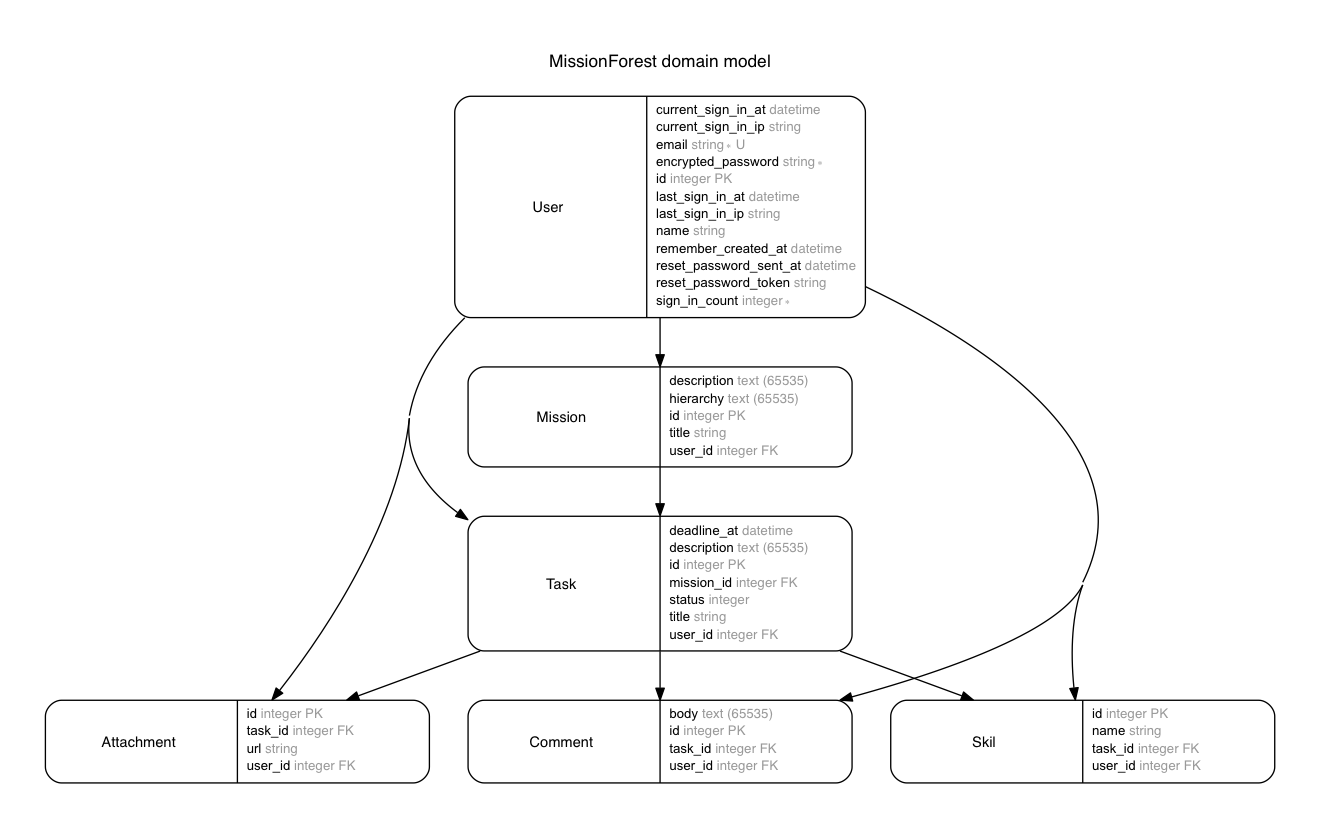
\includegraphics[width=0.9\linewidth]{assets/img/system_model.png}
		\caption{データベースER図}
		\label{img:system_model}
	\end{center}
\end{figure}
